\documentclass[
11pt, % The default document font size, options: 10pt, 11pt, 12pt
codirector, % Uncomment to add a codirector to the title page
]{charter} 


% El títulos de la memoria, se usa en la carátula y se puede usar el cualquier lugar del documento con el comando \ttitle
\titulo{Estación de radio portátil para el monitoreo de radioemisiones comerciales} 

% Nombre del posgrado, se usa en la carátula y se puede usar el cualquier lugar del documento con el comando \degreename
\posgrado{Carrera de Especialización en Sistemas Embebidos} 
%\posgrado{Carrera de Especialización en Internet de las Cosas} 
%\posgrado{Carrera de Especialización en Inteligencia Artificial}
%\posgrado{Maestría en Sistemas Embebidos} 
%\posgrado{Maestría en Internet de las cosas}
% IMPORTANTE: no omitir titulaciones ni tildación en los nombres, también se recomienda escribir los nombres completos (tal cual los tienen en su documento)
% Tu nombre, se puede usar el cualquier lugar del documento con el comando \authorname
\autor{Ramiro Sanes}

% El nombre del director y co-director, se puede usar el cualquier lugar del documento con el comando \supname y \cosupname y \pertesupname y \pertecosupname
\director{Pablo Iturralde}
\pertenenciaDirector{UCU} 
\codirector{FirmWareSpecialist} % para que aparezca en la portada se debe descomentar la opción codirector en los parámetros de documentclass
\pertenenciaCoDirector{FIUBA}

% Nombre del cliente, quien va a aprobar los resultados del proyecto, se puede usar con el comando \clientename y \empclientename
\cliente{Pablo Iturralde}
\empresaCliente{UCU}
 
\fechaINICIO{20 de agosto de 2024}		%Fecha de inicio de la cursada de GdP \fechaInicioName
\fechaFINALPlan{8 de octubre de 2024} 	%Fecha de final de cursada de GdP
\fechaFINALTrabajo{20 de junio de 2025}	%Fecha de defensa pública del trabajo final


\begin{document}

\maketitle
\thispagestyle{empty}
\pagebreak


\thispagestyle{empty}
{\setlength{\parskip}{0pt}
\tableofcontents{}
}
\pagebreak


\section*{Registros de cambios}
\label{sec:registro}


\begin{table}[ht]
\label{tab:registro}
\centering
\begin{tabularx}{\linewidth}{@{}|c|X|c|@{}}
\hline
\rowcolor[HTML]{C0C0C0} 
Revisión & \multicolumn{1}{c|}{\cellcolor[HTML]{C0C0C0}Detalles de los cambios realizados} & Fecha      \\ \hline
0      & Creación del documento                                 &\fechaInicioName \\ \hline
1      & Se completa hasta el punto 5 inclusive                & {2} de {setiembre} de 2024 \\ \hline
%2      & Se completa hasta el punto 9 inclusive
%		  Se puede agregar algo más \newline
%		  En distintas líneas \newline
%		  Así                                                    & {día} de {mes} de 202X \\ \hline
%3      & Se completa hasta el punto 12 inclusive                & {día} de {mes} de 202X \\ \hline
%4      & Se completa el plan	                                 & {día} de {mes} de 202X \\ \hline

% Si hay más correcciones pasada la versión 4 también se deben especificar acá

\end{tabularx}
\end{table}

\pagebreak



\section*{Acta de constitución del proyecto}
\label{sec:acta}

\begin{flushright}
Buenos Aires, \fechaInicioName
\end{flushright}

\vspace{2cm}

Por medio de la presente se acuerda con \authorname\hspace{1px} que su Trabajo Final de la \degreename\hspace{1px} se titulará ``\ttitle'' y consistirá en la implementación de un dispositivo portátil y de bajo costo para el monitoreo de estaciones de radios FM. El trabajo tendrá un presupuesto preliminar estimado de 600 horas y un costo estimado de {\$ 200}, con fecha de inicio el \fechaInicioName\hspace{1px} y fecha de presentación pública en junio de 2025.

Se adjunta a esta acta la planificación inicial.

\vfill

% Esta parte se construye sola con la información que hayan cargado en el preámbulo del documento y no debe modificarla
\begin{table}[ht]
\centering
\begin{tabular}{ccc}
\begin{tabular}[c]{@{}c@{}}Dr. Ing. Ariel Lutenberg \\ Director posgrado FIUBA\end{tabular} & \hspace{2cm} & \begin{tabular}[c]{@{}c@{}}\clientename \\ \empclientename \end{tabular} \vspace{2.5cm} \\ 
\multicolumn{3}{c}{\begin{tabular}[c]{@{}c@{}} \supname \\ Director del Trabajo Final\end{tabular}} \vspace{2.5cm} \\
\end{tabular}
\end{table}

\section{1. Descripción técnica-conceptual del proyecto a realizar}
\label{sec:descripcion}
\textbf{Contexto}

El control y la regulación de las emisiones de las bandas de FM es esencial para garantizar la calidad del servicio, detectar interferencias o asegurar el cumplimiento de las normas, por establecer unos primeros ejemplos. En Uruguay, el organismo encargado de estas normas es la URSEC (Unidad Reguladora de Servicios de Energía y Comunicaciones). Los equipos utilizados para estos fines suelen ser sofisticados, complejos y costosos. 

Por otro lado, desde hace algunos años existen en el mercado periféricos llamados RTL-SDR. Estos dispositivos son de bajo costo y tamaño, y pueden sintonizarse en diversas bandas del espectro electromagnético (VHF). Además, cuentan con un ancho de banda y una velocidad de transferencia suficientes para realizar el procesamiento o la demodulación de las señales mediante software. Se encuentran en el mercado diversos RTL-SDR en el entorno de los 50 USD, de diversos fabricantes y características operativas muy similares.

\begin{figure}[H]
\centering 
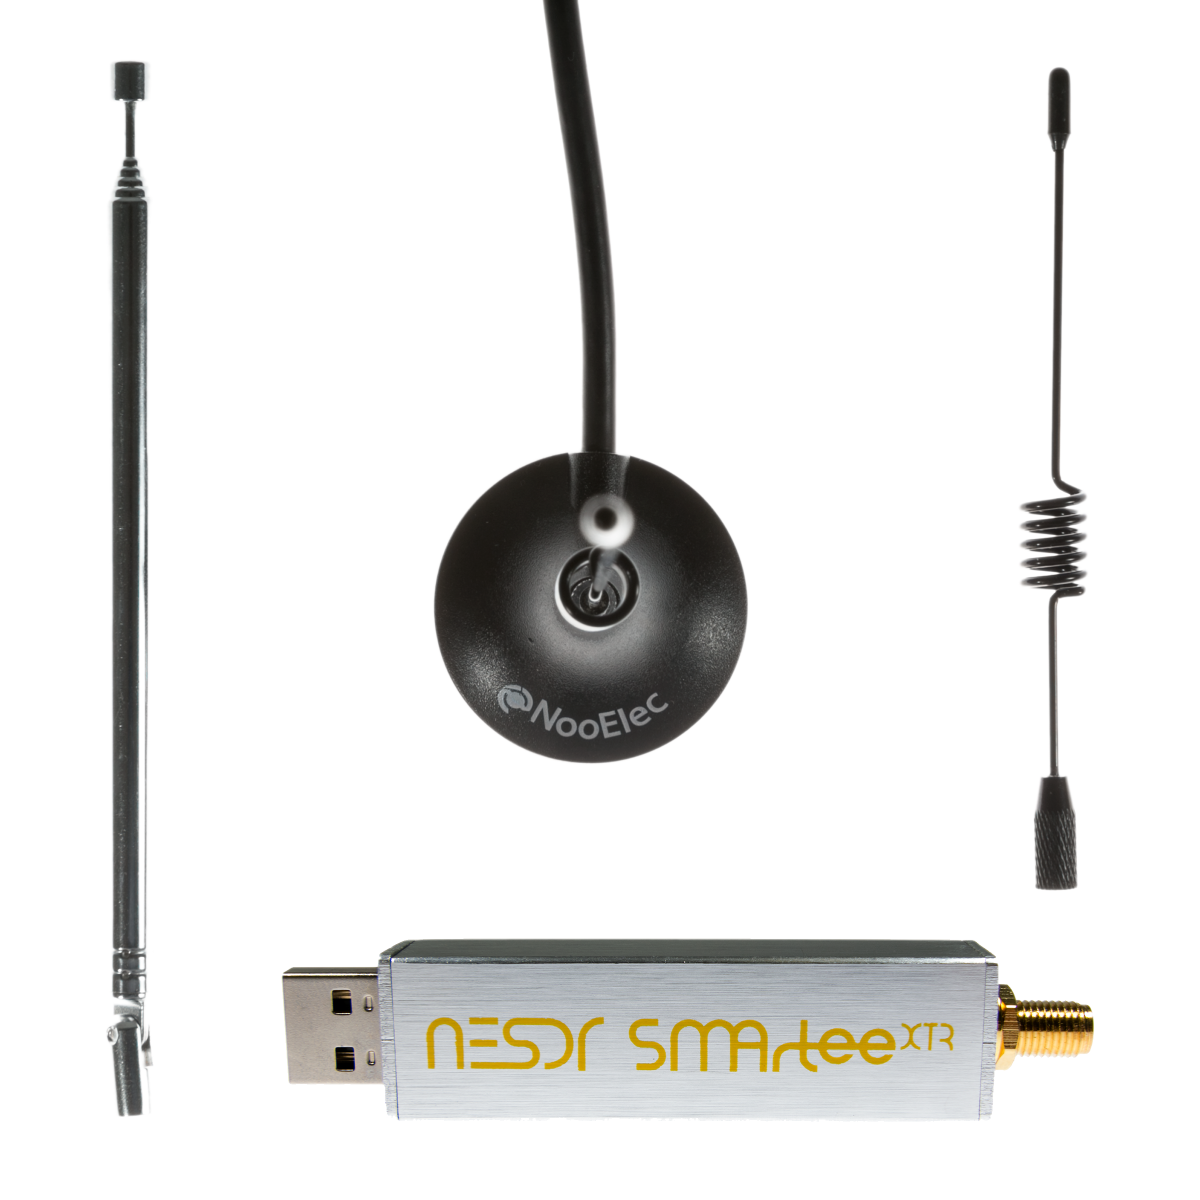
\includegraphics[width=.65\textwidth]{./Figuras/RTL-SDR.png} 
\caption{Nooelec SDR Bundle: RTL-SDR y antenas.}
\label{fig:diagBloques}
\end{figure}

En los últimos años, la Raspberry Pi ha ganado popularidad como herramienta para implementar proyectos de bajo costo y fácil acceso. Gracias a su versatilidad y amplia documentación disponible, se utilizará en este trabajo para conectar diversos tipos de hardware de visualización de datos, así como para integrar y gestionar interfaces USB necesarias para la operación del sistema

En el presente trabajo se pretende desarrollar una estación de recepción de radio portátil que permita a sus usuarios configurarlo para realizar diversas tareas de monitoreo, en las emisiones de radio comerciales más comunes, en particular la banda FM (80-120 MHz). Este dispositivo será fácilmente replicable con tecnologías OTS (Of The Shelf) y open source, para hacerlo de bajo costo y fácil despliegue. 

\begin{figure}[H]
\centering 
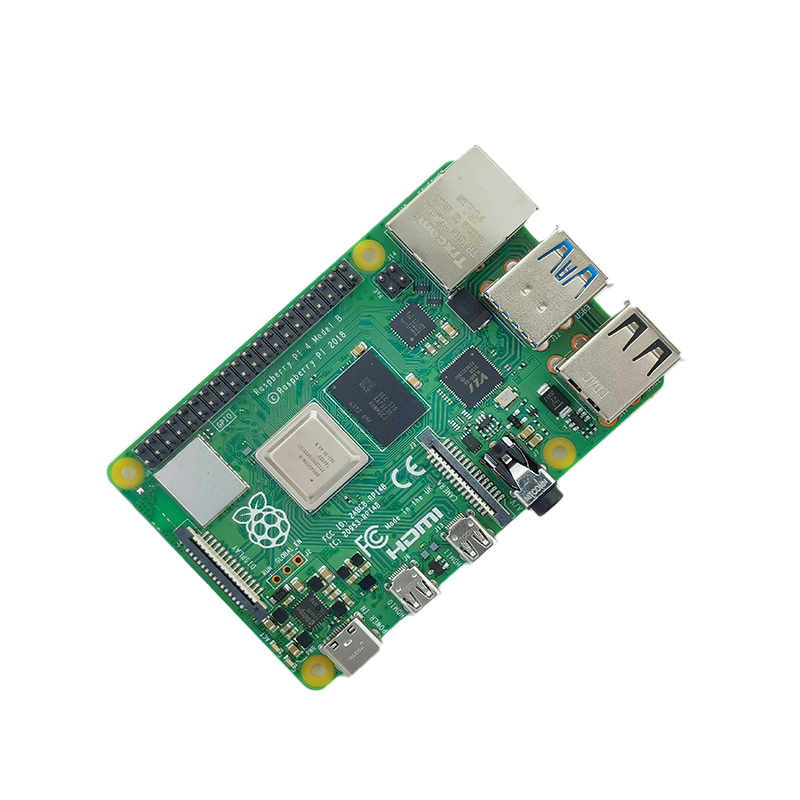
\includegraphics[width=.65\textwidth]{./Figuras/Raspi4B.png} 
\caption{Raspberry Pi model 4B.}
\label{fig:diagBloques}
\end{figure}

Es un trabajo que integra diversos aspectos del manejo de periféricos y de sistemas para poder realizar una tarea específica, que es de interés particular para un ente regulador, pero también para radioaficionados. Además profundiza en el conocimiento de la fenomenología RF y sus aplicaciones prácticas en la electrónica. Involucra conocimientos en diversas áreas, tanto en hardware, como en software, ciencias aplicadas y gestión de proyectos.

Es deseable que este dispositivo pueda ser accedible remotamente, para poder leer o guardar su información en tiempo real, como también es óptimo que tenga la capacidad de algún tipo de interfaz para la visualización de datos espectrales. En principio, estos requerimientos pueden modificarse o adaptarse a las necesidades del cliente a medida que se desarrolla el trabajo. 

\textbf{Tecnología}

Se dispone con el hardware adecuado para la implementación de un prototipo inicial y las horas de ingeniería de un estudiante, que pretende ampliar su conocimiento en el desarrollo de electrónica práctica y conocimientos en RF. El hardware consiste en un RTL-SDR (Nooelec Smart Tee Xtr) y una Raspberry Pi 4B. Además, se cuenta con un conocimiento inicial básico de las tecnologías mencionadas, el que pretende ir desarrollándose en profundidad en conjunto con el proyecto. En principio, la elección del hardware inicial no debería cambiar sustancialmente las características del proyecto.

El RTL-SDR, un receptor de radio definido por software (Software Defined Radio), permite sintonizar y demodular una amplia gama de frecuencias, y convierte señales de radio en datos digitales. Este dispositivo cuenta con un Tuner (E4000) y con un demodulador/serializador USB (Realtek R2832U). El funcionamiento interno del dispositivo queda por fuera del alcance de este proyecto, aunque es importante resaltar que es necesario para poder comprender cómo usar la tecnología eficientemente. En el siguiente diagrama de bloques se puede visualizar su funcionamiento a nivel abstracto:

\begin{figure}[h]
\centering 
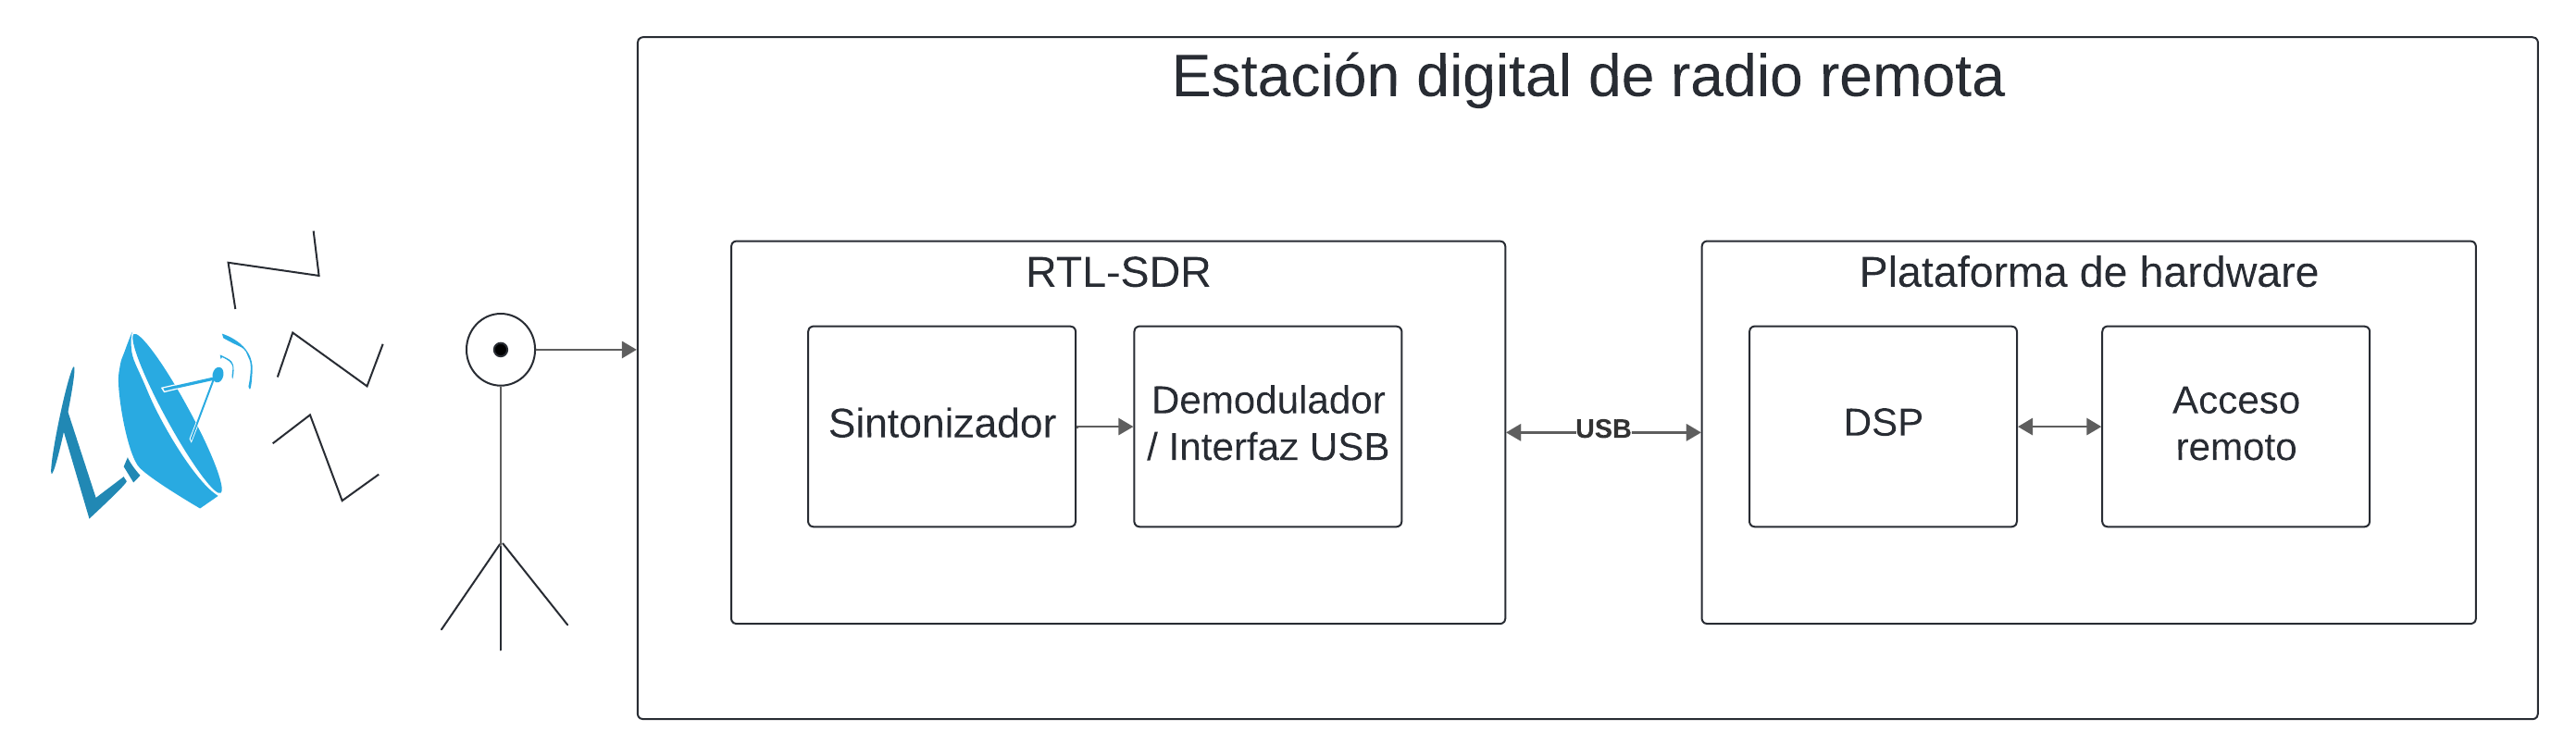
\includegraphics[width=.85\textwidth]{./Figuras/blocksUBA.png} 
\caption{Diagrama funcional del sistema.}
\label{fig:diagBloques}
\end{figure}

Con un dispositivo RTL-SDR y utilizando software, es posible sintonizarse a una estación de radio FM y capturar la información necesaria, como por ejemplo, escuchar el audio codificado en ellas o medir el nivel de intensidad de la emisión. Estas funcionalidades están ampliamente documentadas. Además, existen diversas aplicaciones para radioaficionados que permiten explorar rápidamente las posibilidades de un SDR. Por ejemplo, es posible visualizar el espectro electromagnético de manera gráfica.

\textbf{Resumen}

Este proyecto explorará diferentes enfoques para adquirir la mayor cantidad de información posible sobre las emisiones en la banda FM utilizando SDR en la plataforma Raspberry Pi. Se evaluará tanto la optimización de las capacidades del periférico como de la arquitectura, con el objetivo de capturar la mayor cantidad de información relevante.


\section{2. Identificación y análisis de los interesados}
\label{sec:interesados}

\begin{table}[ht]
%\caption{Identificación de los interesados}
%\label{tab:interesados}
\begin{tabularx}{\linewidth}{@{}|l|X|X|l|@{}}
\hline
\rowcolor[HTML]{C0C0C0} 
Rol           & Nombre y Apellido & Organización 	& Puesto 	\\ \hline
Cliente       & \clientename      &\empclientename	&   Director del Trabajo Final \\ \hline
Responsable   & \authorname       & FIUBA        	& Alumno 	\\ \hline
Orientador    & todefine	      & todefine	 	&  Co-director\\ \hline
Cliente    & \clientename	      & URSEC		 	&  Director del Trabajo Final\\ \hline
\end{tabularx}
\end{table}



\section{3. Propósito del proyecto}
\label{sec:proposito}

El propósito de este proyecto es desarrollar una estación portátil de radio digital, para que diversos agentes como radioaficionados o entes reguladores puedan monitorear, escuchar y/o procesar las radioemisiones que se transmiten a los distintos puntos de un territorio, o en el hogar del usuario. 

Esta estación estará embebida en el hardware apropiado y fácilmente adquirible. Inicialmente, será una Raspberry Pi 4B y un Nooelec RTL-SDR. El sistema debe ser fácilmente operable por los agentes que desean obtener información relevante. Además, el sistema debería ser autónomo, es decir, que se pueda colocar en cualquier lugar y realizar tareas de monitoreo específicas, ya sean estándar o personalizadas. Para ello el sistema deberá ser modular y fácilmente escalable, para poder también idear un despliegue de muchas estaciones de radio en simultáneo.

\section{4. Alcance del proyecto}
\label{sec:alcance}

El proyecto abarca la investigación, el diseño y la implementación del prototipo. Para ser más específico, a continuación se itemizan los distintos aspectos:

\begin{itemize}
	\item Implementación de recepción de señales RF con el hardware inicial
		\begin{itemize}
		\item Investigación de fenomenología, sampleo y demodulación RF.
		\item Investigación de drivers.
		\item Investigación de aplicaciones/software existente.
		\end{itemize}
	\item Caracterización de capacidades de hardware y plataforma
		\begin{itemize}
		\item Ancho de banda disponible y necesario.
		\item Consumo de potencia.
		\item Estimación de capacidades máximas de extracción de información relevante según hardware inicial.
		\end{itemize}
	\item Implementación de estación de radio digital
		\begin{itemize}
		\item Desarrollo de software de monitoreo.
		\item Desarrollo de software de visualización de datos.
		\item Desarrollo de geologalización y conectividad remota.
		\item Integración de diversos módulos de software en el sistema final.
		\end{itemize}
	\item Caracterización de sistema final
		\begin{itemize}
		\item Límites de extracción de información del sistema.
		\item Estudio de escalabilidad del sistema final.
		\end{itemize}
\end{itemize}

El proyecto no incluye:
\begin{itemize}
	\item Desarrollo de drivers USB.
	\item Despliegue/Implementación de varias estaciones de radio en simultáneo.
\end{itemize}



\section{5. Supuestos del proyecto}
\label{sec:supuestos}

Para el desarrollo del presente proyecto se supone que:

\begin{itemize}
	\item Se cuenta con el hardware inicial acorde para las necesidades iniciales
		\begin{itemize}
		\item Ancho de banda suficiente para recibir señales de audio de al menos una radio FM en un tiempo dado.
		\item La plataforma seleccionada tiene la capacidad de potencia suficiente para mantener recepciones por tiempos continuos e indefinidos.
		\item Todos los drivers/software necesarios para su operación se encuentran ampliamente disponibles y existen muchas herramientas open source para apoyarse y colaborar.
		\end{itemize}
	\item Los requerimientos y especificaciones irán modificándose a medida que se desarrolle el proyecto.
	\item Se cuenta con el conocimiento y tiempo suficiente para poder implementar estas tecnologías de una manera sofisticada, con buenas prácticas, y que aproveche el máximo el hardware disponible.
\end{itemize}

\section{6. Requerimientos}
\label{sec:requerimientos}

A continuación se listarán los requerimientos que deba cumplir el prototipo a desarrollarse para considerarlo exitoso:

\begin{enumerate}
	\item Requerimientos funcionales:
		\begin{itemize}
			\item El sistema debe poder realizar tareas de monitoreo básico 		autónomamente.
			\item El sistema debe consistir únicamente en partes de hardware OTS y de fácil armado.
			\item Los usuarios deben poder acceder al sistema remotamente para ver información de interés, o para configurar al dispositivo.
			\item El sistema deberá mínimamente ser capaz de capturar la mayor cantidad de información relevante de al menos una emisión de radio FM en un tiempo dado.
		\end{itemize}
	\item Requerimientos de documentación:
		\begin{itemize}
			\item El sistema deberá tener un manual de usuario para poder operarlo tanto en sitio como remotamente, de manera sencilla.
			\item Se debe contar con un documento que caracterize al sistema de tal manera de conocer sus rangos de operación o de extracción de información máxima.
		\end{itemize}
	\item Requerimientos de operabilidad:
		\begin{itemize}
			\item El acceso del sistema remoto debe ser sencillo y con herramientas cotidianas (navegador web o smartphone).
		\end{itemize}
\end{enumerate}

\section{7. Historias de usuarios (\textit{Product backlog})}
\label{sec:backlog}

Se identifican determinados roles para las historias de usuario:

\begin{itemize}
	\item Usuario final (radioaficionados): Estos usuarios son personas sin un conocimiento muy amplio en la electrónica o en el mundo RF. Estos usuarios esperan tener un dispositivo fácilmente adquiribles por ellos y fácilmente operable.
	\item Usuario final (entes reguladores): Estos operadores del dispositivo desean poder obtener diversas métricas de catacterización de las señales obtenidas. Además también van a estar interesados en qué lugar de un territorio se hicieron tales mediciones. Por último, este usuario también desea poder procesar la mayor cantidad de información relevante de manera autónoma, mediante scripts o configuración del sistema.
	\item Proyectante: Como emprendimiento personal, se desea adquirir la mayor cantidad de formación y experiencia posible en los diversos campos que abarcan este proyecto. Se desea implementar un producto finalizado que sea escalable y modular. Se espera tener un conocimiento profundo de todo lo implementado y a la vez abstracto o de alto nivel: Conocimiento desde las operaciones mas simples hasta la interoperabilidad de distintas operaciones trabajando en simultáneo para un sistema final.
\end{itemize}

Para las historias de usuario que se presentan a continuación, se les asigna un punto de historia (\textit{history points}) en tres categorías: dificultad, complejidad y riesgo o incertidumbre. La escala de puntuación es análoga a la sucesión de Fibonacci y la suma de los puntos de historia de cada categoría representa los puntos de historias total (redondeando el número superior más próximo a la sucesión de Fibonacci).


\begin{table}[h]
\centering
\begin{tabular}{|c|c|c|c|} 
\hline
\rowcolor[HTML]{C0C0C0} 
\textbf{Grado} & \textbf{Dificultad} & \textbf{Complejidad} & \textbf{Riesgo o Incertidumbre}\\
\hline
Bajo & 1 & 1 & 1\\ 
\hline
Medio & 3 & 5 & 8\\ 
\hline
Alto & 5 & 13 & 21\\ 
\hline
\end{tabular}
\end{table}

-----------
Descripción: en esta sección se deben incluir las historias de usuarios y su ponderación (\textit{history points}). Recordar que las historias de usuarios son descripciones cortas y simples de una característica contada desde la perspectiva de la persona que desea la nueva capacidad, generalmente un usuario o cliente del sistema. La ponderación es un número entero que representa el tamaño de la historia comparada con otras historias de similar tipo.

Se debe indicar explícitamente el criterio para calcular los \textit{story points} de cada historia.
------


\begin{enumerate}
\item ``Como [rol] quiero [tal cosa] para [tal otra cosa]."

\textit{Story points}: 8 (complejidad: 3, dificultad: 2, incertidumbre: 3)
\end{enumerate}


\section{8. Entregables principales del proyecto}
\label{sec:entregables}

\begin{consigna}{red}
Los entregables del proyecto son (ejemplo):

\begin{itemize}
	\item Manual de usuario.
	\item Diagrama de circuitos esquemáticos.
	\item Código fuente del firmware.
	\item Diagrama de instalación.
	\item Memoria del trabajo final.
	\item etc...
\end{itemize}
\end{consigna}

\section{9. Desglose del trabajo en tareas}
\label{sec:wbs}

\begin{consigna}{red}
El WBS debe tener relación directa o indirecta con los requerimientos.  Son todas las actividades que se harán en el proyecto para dar cumplimiento a los requerimientos. Se recomienda mostrar el WBS mediante una lista indexada:

\begin{enumerate}
\item Grupo de tareas 1 (suma h)
	\begin{enumerate}
	\item Tarea 1 (tantas h)
	\item Tarea 2 (tantas h)
	\item Tarea 3 (tantas h)
	\end{enumerate}
\item Grupo de tareas 2 (suma h)
	\begin{enumerate}
	\item Tarea 1 (tantas h)
	\item Tarea 2 (tantas h)
	\item Tarea 3 (tantas h)
	\end{enumerate}
\item Grupo de tareas 3 (suma h)
	\begin{enumerate}
	\item Tarea 1 (tantas h)
	\item Tarea 2 (tantas h)
	\item Tarea 3 (tantas h)
	\item Tarea 4 (tantas h)
	\item Tarea 5 (tantas h)
	\end{enumerate}
\end{enumerate}

Cantidad total de horas: tantas.

\textbf{¡Importante!:} la unidad de horas es h y va separada por espacio del número. Es incorrecto escribir ``23hs".

\textbf{Se recomienda que no haya ninguna tarea que lleve más de 40 h.} De ser así se recomienda dividirla en tareas de menor duración.

\end{consigna}

\section{10. Diagrama de Activity On Node}
\label{sec:AoN}

\begin{consigna}{red}
Armar el AoN a partir del WBS definido en la etapa anterior.

Una herramienta simple para desarrollar los diagramas es el Draw.io (\url{https://app.diagrams.net/}).
\href{https://app.diagrams.net}{Draw.io}


\begin{figure}[htpb]
\centering 
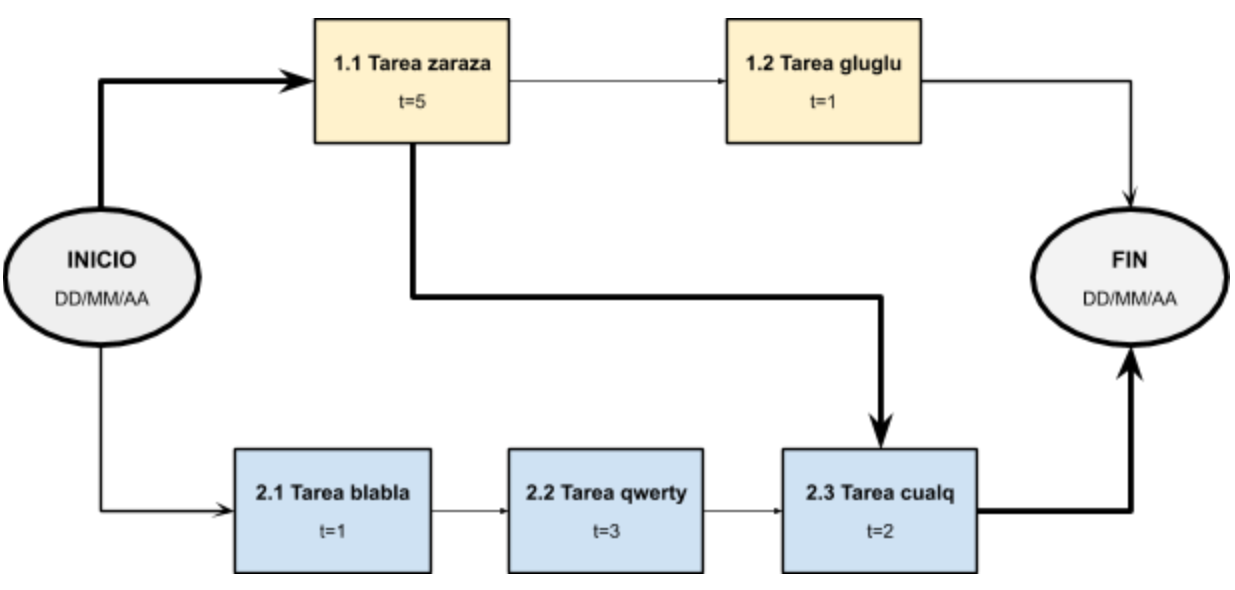
\includegraphics[width=.8\textwidth]{./Figuras/AoN.png}
\caption{Diagrama de \textit{Activity on Node}.}
\label{fig:AoN}
\end{figure}

Indicar claramente en qué unidades están expresados los tiempos.
De ser necesario indicar los caminos semi críticos y analizar sus tiempos mediante un cuadro.
Es recomendable usar colores y un cuadro indicativo describiendo qué representa cada color.

\end{consigna}

\section{11. Diagrama de Gantt}
\label{sec:gantt}

\begin{consigna}{red}
Existen muchos programas y recursos \textit{online} para hacer diagramas de Gantt, entre los cuales destacamos:

\begin{itemize}
\item Planner
\item GanttProject
\item Trello + \textit{plugins}. En el siguiente link hay un tutorial oficial: \\ \url{https://blog.trello.com/es/diagrama-de-gantt-de-un-proyecto}
\item Creately, herramienta online colaborativa. \\\url{https://creately.com/diagram/example/ieb3p3ml/LaTeX}
\item Se puede hacer en latex con el paquete \textit{pgfgantt}\\ \url{http://ctan.dcc.uchile.cl/graphics/pgf/contrib/pgfgantt/pgfgantt.pdf}
\end{itemize}

Pegar acá una captura de pantalla del diagrama de Gantt, cuidando que la letra sea suficientemente grande como para ser legible. 
Si el diagrama queda demasiado ancho, se puede pegar primero la ``tabla'' del Gantt y luego pegar la parte del diagrama de barras del diagrama de Gantt.

Configurar el software para que en la parte de la tabla muestre los códigos del EDT (WBS).\\
Configurar el software para que al lado de cada barra muestre el nombre de cada tarea.\\
Revisar que la fecha de finalización coincida con lo indicado en el Acta Constitutiva.

En la figura \ref{fig:gantt}, se muestra un ejemplo de diagrama de gantt realizado con el paquete de \textit{pgfgantt}. 
En la plantilla pueden ver el código que lo genera y usarlo de base para construir el propio.

Las fechas pueden ser calculadas utilizando alguna de las herramientas antes citadas. Sin embargo, el siguiente ejemplo
fue elaborado utilizando 
\href{https://docs.google.com/spreadsheets/d/1fBz8NhSpc4tkkhz3KjJCbh1nR_ltDkfEcZi4tZXduqs}{esta hoja de cálculo}.

Es importante destacar que el ancho del diagrama estará dado por la longitud del texto utilizado para las tareas 
(Ejemplo: tarea 1, tarea 2, etcétera) y el valor \textit{x unit}. Para mejorar la apariencia del diagrama, es necesario
ajustar este valor y, quizás, acortar los nombres de las tareas.

\begin{figure}[htpb]
  \begin{center}
    \begin{ganttchart}[
      time slot unit=day,
      time slot format=isodate,
      x unit=0.038cm,
      y unit title=0.7cm,
      y unit chart=0.6cm,
      milestone/.append style={xscale=4}
      ]{2021-03-05}{2021-12-16}
      \gantttitlecalendar*{2021-03-05}{2021-12-16}{year} \\
      \gantttitlecalendar*{2021-03-05}{2021-12-16}{month} \\
      \ganttgroup{Duración Total}{2021-03-05}{2021-12-16} \\
      %%%%%%%%%%%%%%%%%Organización
      \ganttgroup{Organización}{2021-03-05}{2021-04-16} \\
      \ganttbar{Planificación del proyecto}{2021-03-05}{2021-04-15} \\
      %%%%%%%%%%%%%%%%%Ejecución
      \ganttgroup{Ejecución}{2021-04-16}{2021-10-21} \\
      \ganttbar{Tarea 1}{2021-04-16}{2021-04-29} \\
      \ganttbar{Tarea 2}{2021-04-30}{2021-05-13} \\
      \ganttbar{Tarea 3}{2021-05-14}{2021-05-27} \\
      \ganttbar{Tarea 4}{2021-05-28}{2021-07-12} \\
      \ganttbar{Tarea 5}{2021-07-13}{2021-08-09} \\
      \ganttbar{Tarea 6}{2021-08-10}{2021-09-23} \\
      \ganttbar{Tarea 7}{2021-09-24}{2021-09-30} \\
      \ganttbar{Tarea 8}{2021-10-01}{2021-10-14} \\
      \ganttbar{Tarea 9}{2021-10-15}{2021-10-21} \\
      % %%%%%%%%%%%%%%%%%Finalización
      \ganttgroup{Finalización}{2021-10-22}{2021-12-16} \\
      \ganttbar{Memoria v1}{2021-10-22}{2021-11-04} \\
      \ganttbar{Memoria v2}{2021-11-05}{2021-11-18} \\
      \ganttbar{Memoria final}{2021-11-19}{2021-12-02} \\
      % La fecha del siguiente milestone es la fecha en que terminamos la memoria
      \ganttmilestone{Enviar memoria al director}{2021-12-02} \\
      \ganttbar{Elaborar la presentación}{2021-12-03}{2021-12-16} \\
      \ganttmilestone{Ensayo de la presentación}{2021-12-16} \\
      %%%%%%%%%%%%%%%%%%%%%%%%%%%%%%%%%%%%%%%%%%%%%%%%%%%%%%%%%%%%%%%
    \end{ganttchart}
  \end{center}
  \caption{Diagrama de gantt de ejemplo}
  \label{fig:gantt}
\end{figure}


\begin{landscape}
\begin{figure}[htpb]
\centering 
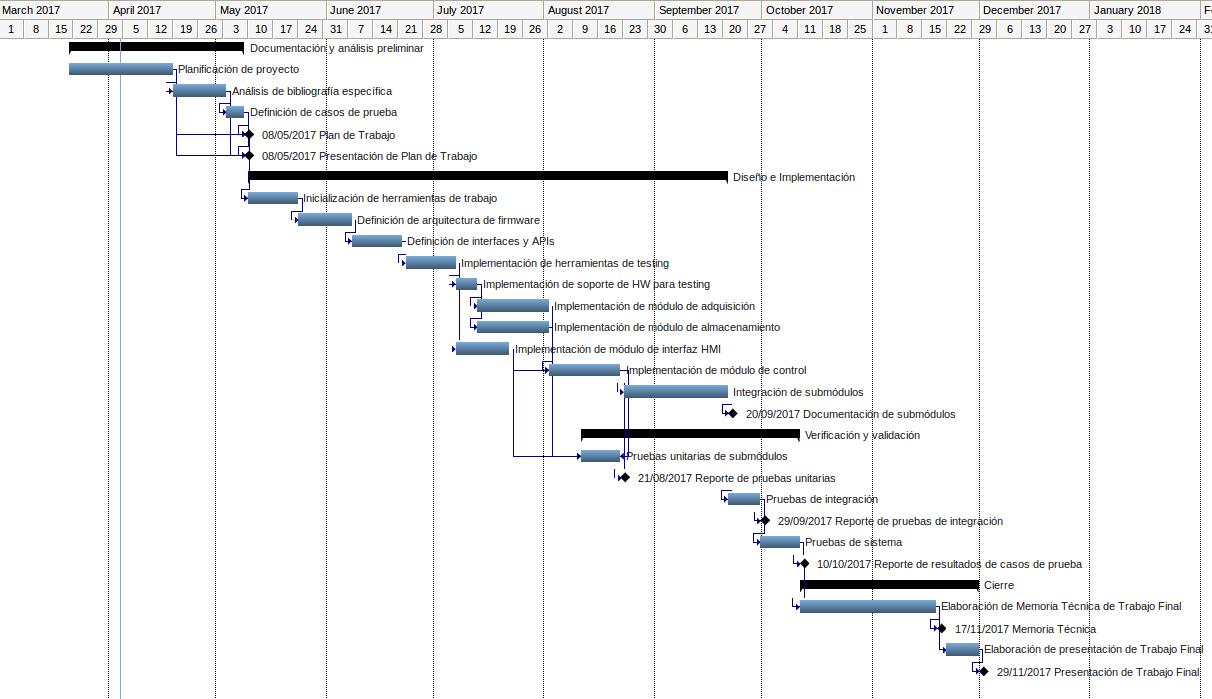
\includegraphics[height=.85\textheight]{./Figuras/Gantt-2.png}
\caption{Ejemplo de diagrama de Gantt (apaisado).} %Modificar este título acorde.
\label{fig:diagGantt}
\end{figure}

\end{landscape}

\end{consigna}


\section{12. Presupuesto detallado del proyecto}
\label{sec:presupuesto}

\begin{consigna}{red}
Si el proyecto es complejo entonces separarlo en partes:
\begin{itemize}
	\item Un total global, indicando el subtotal acumulado por cada una de las áreas.
	\item El desglose detallado del subtotal de cada una de las áreas.
\end{itemize}

IMPORTANTE: No olvidarse de considerar los COSTOS INDIRECTOS.

Incluir la aclaración de si se emplea como moneda el peso argentino (ARS) o si se usa moneda extranjera (USD, EUR, etc). Si es en moneda extranjera se debe indicar la tasa de conversión respecto a la moneda local en una fecha dada.

\end{consigna}

\begin{table}[htpb]
\centering
\begin{tabularx}{\linewidth}{@{}|X|c|r|r|@{}}
\hline
\rowcolor[HTML]{C0C0C0} 
\multicolumn{4}{|c|}{\cellcolor[HTML]{C0C0C0}COSTOS DIRECTOS} \\ \hline
\rowcolor[HTML]{C0C0C0} 
Descripción &
  \multicolumn{1}{c|}{\cellcolor[HTML]{C0C0C0}Cantidad} &
  \multicolumn{1}{c|}{\cellcolor[HTML]{C0C0C0}Valor unitario} &
  \multicolumn{1}{c|}{\cellcolor[HTML]{C0C0C0}Valor total} \\ \hline
 &
  \multicolumn{1}{c|}{} &
  \multicolumn{1}{c|}{} &
  \multicolumn{1}{c|}{} \\ \hline
 &
  \multicolumn{1}{c|}{} &
  \multicolumn{1}{c|}{} &
  \multicolumn{1}{c|}{} \\ \hline
\multicolumn{1}{|l|}{} &
   &
   &
   \\ \hline
\multicolumn{1}{|l|}{} &
   &
   &
   \\ \hline
\multicolumn{3}{|c|}{SUBTOTAL} &
  \multicolumn{1}{c|}{} \\ \hline
\rowcolor[HTML]{C0C0C0} 
\multicolumn{4}{|c|}{\cellcolor[HTML]{C0C0C0}COSTOS INDIRECTOS} \\ \hline
\rowcolor[HTML]{C0C0C0} 
Descripción &
  \multicolumn{1}{c|}{\cellcolor[HTML]{C0C0C0}Cantidad} &
  \multicolumn{1}{c|}{\cellcolor[HTML]{C0C0C0}Valor unitario} &
  \multicolumn{1}{c|}{\cellcolor[HTML]{C0C0C0}Valor total} \\ \hline
\multicolumn{1}{|l|}{} &
   &
   &
   \\ \hline
\multicolumn{1}{|l|}{} &
   &
   &
   \\ \hline
\multicolumn{1}{|l|}{} &
   &
   &
   \\ \hline
\multicolumn{3}{|c|}{SUBTOTAL} &
  \multicolumn{1}{c|}{} \\ \hline
\rowcolor[HTML]{C0C0C0}
\multicolumn{3}{|c|}{TOTAL} &
   \\ \hline
\end{tabularx}%
\end{table}


\section{13. Gestión de riesgos}
\label{sec:riesgos}

\begin{consigna}{red}
a) Identificación de los riesgos (al menos cinco) y estimación de sus consecuencias:
 
Riesgo 1: detallar el riesgo (riesgo es algo que si ocurre altera los planes previstos de forma negativa)
\begin{itemize}
	\item Severidad (S): mientras más severo, más alto es el número (usar números del 1 al 10).\\
	Justificar el motivo por el cual se asigna determinado número de severidad (S).
	\item Probabilidad de ocurrencia (O): mientras más probable, más alto es el número (usar del 1 al 10).\\
	Justificar el motivo por el cual se asigna determinado número de (O). 
\end{itemize}   

Riesgo 2:
\begin{itemize}
	\item Severidad (S): X.\\
	Justificación...
	\item Ocurrencia (O): Y.\\
	Justificación...
\end{itemize}

Riesgo 3:
\begin{itemize}
	\item Severidad (S):  X.\\
	Justificación...
	\item Ocurrencia (O): Y.\\
	Justificación...
\end{itemize}


b) Tabla de gestión de riesgos:      (El RPN se calcula como RPN=SxO)

\begin{table}[htpb]
\centering
\begin{tabularx}{\linewidth}{@{}|X|c|c|c|c|c|c|@{}}
\hline
\rowcolor[HTML]{C0C0C0} 
Riesgo & S & O & RPN & S* & O* & RPN* \\ \hline
       &   &   &     &    &    &      \\ \hline
       &   &   &     &    &    &      \\ \hline
       &   &   &     &    &    &      \\ \hline
       &   &   &     &    &    &      \\ \hline
       &   &   &     &    &    &      \\ \hline
\end{tabularx}%
\end{table}

Criterio adoptado: 

Se tomarán medidas de mitigación en los riesgos cuyos números de RPN sean mayores a...

Nota: los valores marcados con (*) en la tabla corresponden luego de haber aplicado la mitigación.

c) Plan de mitigación de los riesgos que originalmente excedían el RPN máximo establecido:
 
Riesgo 1: plan de mitigación (si por el RPN fuera necesario elaborar un plan de mitigación).
  Nueva asignación de S y O, con su respectiva justificación:
  \begin{itemize}
	\item Severidad (S*): mientras más severo, más alto es el número (usar números del 1 al 10).
          Justificar el motivo por el cual se asigna determinado número de severidad (S).
	\item Probabilidad de ocurrencia (O*): mientras más probable, más alto es el número (usar del 1 al 10).
          Justificar el motivo por el cual se asigna determinado número de (O).
	\end{itemize}

Riesgo 2: plan de mitigación (si por el RPN fuera necesario elaborar un plan de mitigación).
 
Riesgo 3: plan de mitigación (si por el RPN fuera necesario elaborar un plan de mitigación).

\end{consigna}


\section{14. Gestión de la calidad}
\label{sec:calidad}

\begin{consigna}{red}
Elija al menos diez requerimientos que a su criterio sean los más importantes/críticos/que aportan más valor y para cada uno de ellos indique las acciones de verificación y validación que permitan asegurar su cumplimiento.

\begin{itemize} 
\item Req \#1: copiar acá el requerimiento con su correspondiente número.

\begin{itemize}
	\item Verificación para confirmar si se cumplió con lo requerido antes de mostrar el sistema al cliente. Detallar.
	\item Validación con el cliente para confirmar que está de acuerdo en que se cumplió con lo requerido. Detallar. 
\end{itemize}

\end{itemize}

Tener en cuenta que en este contexto se pueden mencionar simulaciones, cálculos, revisión de hojas de datos, consulta con expertos, mediciones, etc.  

Las acciones de verificación suelen considerar al entregable como ``caja blanca'', es decir se conoce en profundidad su funcionamiento interno.  

En cambio, las acciones de validación suelen considerar al entregable como ``caja negra'', es decir, que no se conocen los detalles de su funcionamiento interno.

\end{consigna}

\section{15. Procesos de cierre}    
\label{sec:cierre}

\begin{consigna}{red}
Establecer las pautas de trabajo para realizar una reunión final de evaluación del proyecto, tal que contemple las siguientes actividades:

\begin{itemize}
	\item Pautas de trabajo que se seguirán para analizar si se respetó el Plan de Proyecto original:\\
	 - Indicar quién se ocupará de hacer esto y cuál será el procedimiento a aplicar. 
	\item Identificación de las técnicas y procedimientos útiles e inútiles que se emplearon, los problemas que surgieron y cómo se solucionaron:\\
	 - Indicar quién se ocupará de hacer esto y cuál será el procedimiento para dejar registro.
	\item Indicar quién organizará el acto de agradecimiento a todos los interesados, y en especial al equipo de trabajo y colaboradores:\\
	  - Indicar esto y quién financiará los gastos correspondientes.
\end{itemize}

\end{consigna}

\end{document}
